\documentclass[12pt, a4paper, oneside]{ctexart}
\usepackage{amsmath, amsthm, amssymb, bm, color, framed, graphicx, hyperref, mathrsfs, float}

% multi-column
\usepackage{tasks}
% itemize
\NewTasksEnvironment[label=(\arabic*), label-width=3ex]{exercise}

\everymath{\displaystyle}

\title{\textbf{第二次作业}}
\author{U08M11002 Spring 2022}
\date{提交截止日期:北京时间2022年3月14日课上(星期一)}
\linespread{1}
\definecolor{shadecolor}{RGB}{241, 241, 255}

\newcounter{problemname}
\newenvironment{problem}{\stepcounter{problemname}\par\noindent\textbf{题目\arabic{problemname}. }}{\\\par}
\newenvironment{warning}{\begin{shaded}\par\noindent\textbf{提交作业方式:}}{\end{shaded}\par}

\begin{document}

\maketitle

\begin{warning}
	从第二次作业开始,需要\textbf{在上课时现场提交纸质版作业}。
	\begin{enumerate}
   	\item 超过截止日期提交的作业按照 0 分计算;
   	\item 截止日期前提交的作业若不符合上述要求,或没有被成功接收,视作没有提交作业。
   	\item 为了你自己复习需要,\textbf{建议上交前自行扫描备份}。
   \end{enumerate}
\end{warning}

\hspace{1em}


\begin{problem}
$a,b \in \mathbb{R}, a \neq 0$,证明:
$$  \int_{-\infty}^{\infty} f(t) \delta(at-b) dt = \frac{1}{|a|} f(\frac{b}{a}) $$
\quad
\end{problem}


\begin{problem}
证明  $\int_{-\infty}^{\infty} f(t) \delta(t-t_0) dt = f(t_0)$.
\quad
\end{problem}

\begin{problem}
证明  $\int_{-\infty}^{\infty} f(t) \delta'(t) dt = -f'(0)$.
\quad
\end{problem}

\begin{problem}
证明:微分、积分和延时器($y(t) = f(t-t_0)$)都是线性系统。
\quad
\end{problem}

\newpage

\begin{problem}
证明以下系统\textbf{不是}时变系统:
\begin{exercise}(2)
	\task (变系数)$y=tf(t)$
	\task (反转)$y=f(-t)$
	\task (伸缩)$y=f(\alpha t)$
\end{exercise}
\quad
\end{problem}


\begin{problem}
判断下列系统的因果性:
\begin{exercise}(2)
	\task $y(t) = f(t-2)$
	\task $y(t) = f(t+2)$
\end{exercise}
\quad
\end{problem}


\begin{problem}
判断下列系统是否为线性的、时不变的、因果的。假设系统均为零状态系统 。
\begin{exercise}(2)
	\task $y(t) = \frac{d^2}{d^2t} f(t)$
	\task $y(t) = f(t) U(t)$
	\task $y(t) = \sin[f(t)] U(t)$
	\task $y(t) = f(1-t)$
	\task $y(t) = f(2t) $
	\task $y(t) = f^2(t) $
	\task $y(t) = \int_{-\infty}^{t} f(\tau) d\tau $
	\task $y(t) = \int_{-\infty}^{5t} f(\tau) d\tau $
\end{exercise}
\quad
\end{problem}

\begin{problem}
线性时不变系统,当激励$f_1(t) = U(t)$ 时,响应 $y_1(t) = e^{-at} U(t)$。试求当激励$f_2(t) = \delta(t)$ 时,响应 $y_2(t)$的表达式。(假定起始时刻系统无储能。)
\quad
\end{problem}


\begin{problem}
已知系统相应的齐次方程及其对应的 $0_+$ 时刻的状态条件,求系统的零输入响应。
\begin{exercise}(1)
	\task $\frac{d^2}{d^2t} y(t) + 2 \frac{d}{dt} y(t) + 2y(t) = 0$,$r(0_+)=1,r'(0_+)=2$
	\task $\frac{d^2}{d^2t} y(t) + 2 \frac{d}{dt} y(t) + y(t) = 0$,$r(0_+)=1,r'(0_+)=2$
	\task $\frac{d^3}{d^3t} y(t) + 2\frac{d^2}{d^2t} y(t) +  \frac{d}{dt} y(t) + 2y(t) = 0 $,$r(0_+)=r'(0_+)=0,r''(0_+)=1 $
\end{exercise}
\quad
\end{problem}

\newpage

\begin{problem}
如下图所示的 RC 电路中,已知 $R = 1 \Omega, C=0.5F$,写出描述该系统的微分方程。电容的初始状态 $u_{C}(0_-) = u_{C}(0_+) = -1V$, 求激励 $u_s(t)$ 为下列信号时的电容 $C$ 的电压全响应 $u_C(t)$:
\begin{figure}[H]
	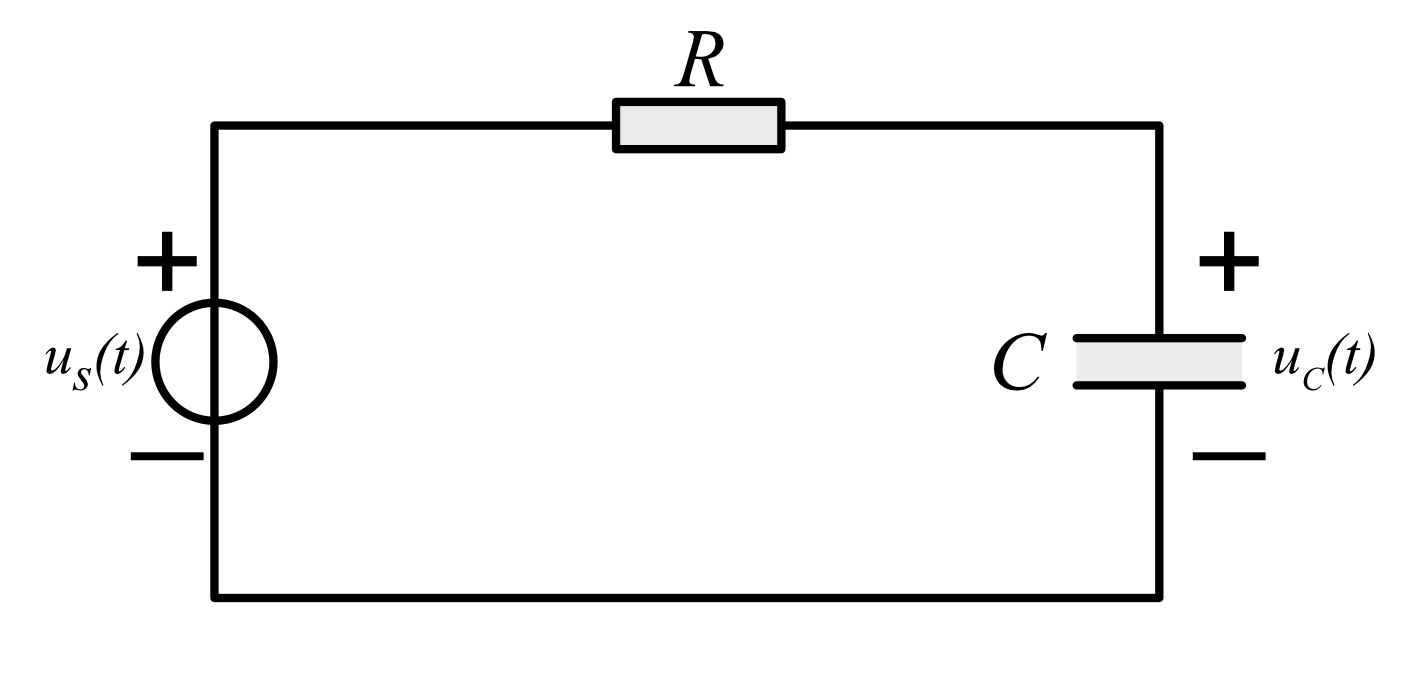
\includegraphics[width=8cm]{assets/hw2img1.png}
	\centering
\end{figure}
\begin{exercise}(2)
	\task $u_s(t) = U(t)$
	\task $u_s(t) = e^{-t}U(t)$
	\task $u_s(t) = e^{-2t}U(t)$
	\task $u_s(t) = tU(t)$
\end{exercise}
\quad
\end{problem}

\end{document}